% Opening packages ---------------------------------

\documentclass[12pt, a4paper]{article}
\parindent 0px
\parskip=10pt
\usepackage[utf8]{vietnam}
\usepackage[left=1.20cm, right=1.20cm, top=1.50cm, bottom=1.50cm]{geometry}
\usepackage{amsmath,amssymb,amsfonts}
\usepackage{gensymb}
\usepackage{enumitem}
\usepackage{multicol}
\usepackage{graphicx}
\usepackage{array}
\usepackage{float}
\usepackage[onehalfspacing]{setspace}
\usepackage{mathpazo}
\usepackage{wrapfig}
\usepackage{tkz-tab}

% Title --------------------------------------------


\title{\vspace{-1.5cm}{\huge\textbf{Ôn thi cuối kỳ I - Lần 2}}\\[3mm]
		{\LARGE Khối lớp: 12}\\[2mm]
{\normalsize Họ và tên~\rule{3cm}{1pt} \hfill Ngày nhận đề: ~\rule{3cm}{1pt}}\\[4mm]
\hrule
}
\author{}
\date{}

% Bắt đầu đề---------------------------------------

\begin{document}
	\maketitle
	\vspace{-2.15cm}
	
\textbf{Phần I: Câu hỏi trắc nghiệm nhiều phương án lựa chọn} 

\textbf{Câu 1: } Cho hàm số $ f(x) $ có bảng biến thiên:
	\begin{center}
			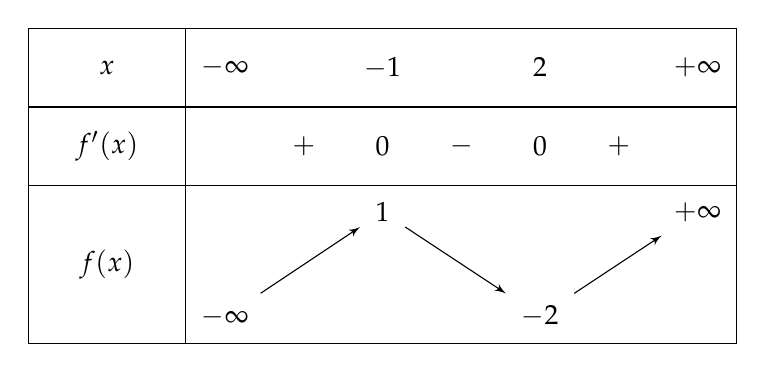
\begin{tikzpicture}
				\tkzTabInit[nocadre = false , lgt = 2 , espcl = 2]
					{ $ x $ / 1 , $ f'(x) $ / 1 , $ f(x) $ / 2 }
					{ $ - \infty $ , $ -1 $ , $ 2 $ , $ + \infty $ } 
				\tkzTabLine
					{ , + , $ 0 $ ,  - , $ 0 $ , + , }
				\tkzTabVar
					{ -/ $ -\infty $ , +/ $ 1 $ , -/ $ -2 $ , +/ $ +\infty $ }
			\end{tikzpicture}
	\end{center}	
	Khẳng định nào sau đây \textbf{sai} ?
	\begin{multicols}{2}
		\begin{enumerate}
			\item[\textbf{A.}] Hàm số đồng biến trên khoảng $ (-2; 1) $
			\item[\textbf{C.}] Hàm số nghịch biến trên khoảng $ (-1; 0 )$
			\item[\textbf{B.}] Hàm số nghịch biến trên khoảng $ (-1; 1) $
			\item[\textbf{D.}] Hàm số đồng biến trên khoảng $ (-2; -1) $
		\end{enumerate}
	\end{multicols}
	

\textbf{Câu 2: } Trong không gian $ Oxyz $, cho $ \vec{a} = (1;2;1) $ và $ \vec{b} = (-1;3;0) $. Véc tơ $ \overrightarrow{c} = 2\vec{a} + \vec{b} $ có tọa độ là
	\begin{multicols}{4}
		\begin{enumerate}
			\item[\textbf{A.}] $ (1; 7; 2) $
			\item[\textbf{B.}] $ (1; 5; 2) $
			\item[\textbf{C.}] $ (3; 7; 2) $
			\item[\textbf{D.}] $ (1; 7; 3) $
		\end{enumerate}
	\end{multicols}

\textbf{Câu 3: } Tìm hiểu thời gian sử dụng điện thoại trong tuần đầu tháng 6/2024 của kỳ nghỉ hè lớp chủ nhiệm GVCN thu được kết quả sau:
	\begin{table}[h!]
		\centering
		\renewcommand{\arraystretch}{1.5}
			\begin{tabular}{|c||c|c|c|c|c|c|}
				\hline
				Thời gian (giờ) & $ [0;5) $ & $ [5; 10) $ & $ [10; 15) $ & $ [15; 20) $ & $ [20; 25) $ & $ [25; 30) $ \\ \hline
				Số học sinh  & 2 & 6  & 8 & 9 & 3 & 2    \\ \hline 
			\end{tabular}
	\end{table}
	
	Khoảng biến thiên của mẫu số liệu ghép nhóm này là
	
	\begin{multicols}{4}
		\begin{enumerate}
			\item[\textbf{A.}] 20
			\item[\textbf{B.}] 25
			\item[\textbf{C.}] 30 
			\item[\textbf{D.}] 15
		\end{enumerate}
	\end{multicols}

\textbf{Câu 4: } Trong không gian $ Oxyz $, hình chiếu vuông góc của điểm $ M(3;1;-1) $ trên trục $ Oy $ có tọa độ là
	\begin{multicols}{4}
		\begin{enumerate}
			\item[\textbf{A.}] $ (3;0;-1) $
			\item[\textbf{B.}] $ (0;1;0) $
			\item[\textbf{C.}] $ (3;0;0) $
			\item[\textbf{D.}] $ (0;0;-1) $
		\end{enumerate}
	\end{multicols}

\pagebreak

\textbf{Câu 5: } Đồ thị hàm số nào sau đây không cắt trục hoành
	\begin{multicols}{2}
		\begin{enumerate}
			\item[\textbf{A.}] $ y = \dfrac{2x - 1}{x + 2} $
			\item[\textbf{C.}] $ y = -x^3 - 2x^2 - 4x + 5 $
			\item[\textbf{B.}] $ y = x^4 + 2x^2 + 3 $
			\item[\textbf{D.}] $ y = -x^4 + 4x^2 - 3 $
		\end{enumerate}
	\end{multicols}

\textbf{Câu 6: } Một mẫu số liệu ghép nhóm có tứ phân vị thứ nhất, thứ hai thứ ba lần lượt là $ Q_1, Q_2, Q_3 $.
	\begin{multicols}{4}
		\begin{enumerate}
			\item[\textbf{A.}] $ \Delta Q = Q_2 - Q_1 $
			\item[\textbf{B.}] $ \Delta Q = Q_3 - Q_1 $
			\item[\textbf{C.}] $ \Delta Q = Q_3 - Q_2 $
			\item[\textbf{D.}] $ \Delta Q = Q_3 + Q_1 $
		\end{enumerate}
	\end{multicols}

\textbf{Câu 7: } Cho hình lập phương $ ABCD.A'B'C'D' $. Tính góc giữa hai vectơ $ \overrightarrow{BC} $ và $ \overrightarrow{B'D'} $
	\begin{multicols}{4}
		\begin{enumerate}
			\item[\textbf{A.}] $ 90 \degree $
			\item[\textbf{B.}] $ 60 \degree $
			\item[\textbf{C.}] $ 45 \degree $
			\item[\textbf{D.}] $ 30 \degree $
		\end{enumerate}
	\end{multicols}

\textbf{Câu 8: } Cho hàm số bậc ba $ y = f(x) $ đạt cực đại tại điểm $ x = 3 $, đạt cực tiểu tại điểm $ x = 0 $. So sánh giá trị $ f(1) $ và $ f(2) $, ta được kết quả nào sau đây?
	\begin{multicols}{4}
		\begin{enumerate}
			\item[\textbf{A.}] $ f(1) < f(2) $
			\item[\textbf{B.}] $ f(1) > f(2) $
			\item[\textbf{C.}] $ f(1) = f(2) $
			\item[\textbf{D.}] Khó rồi
		\end{enumerate}
	\end{multicols}
	
\textbf{Câu 9: } Trong không gian cho điểm $ O $ và bốn điểm $ A, B, C, D $ không thẳng hàng. Điều kiện cần và đủ để $ A, B, C, D $ tạo thành hình bình hành là
	\begin{multicols}{2}
		\begin{enumerate}
			\item[\textbf{A.}] $ \overrightarrow{OA} + \dfrac{1}{2} \overrightarrow{OB} = \overrightarrow{OC} + \dfrac{1}{2} \overrightarrow{OD} $
			\item[\textbf{C.}] $ \overrightarrow{OA} + \dfrac{1}{2} \overrightarrow{OC} = \overrightarrow{OB} + \dfrac{1}{2} \overrightarrow{OD} $
			\item[\textbf{B.}] $ \overrightarrow{OA} + \overrightarrow{OC} = \overrightarrow{OB} + \overrightarrow{OD} $
 			\item[\textbf{D.}] $ \overrightarrow{OA} + \overrightarrow{OB} + \overrightarrow{OC} + \overrightarrow{OD} = \vec{0} $
		\end{enumerate}
	\end{multicols}

\textbf{Câu 10: } Cho hàm số $ f'(x) = x(x - 2), \forall x \in \mathbb{R} $. Giá trị nhỏ nhất của hàm số $ y = f(x) $ trên đoạn $ [1;4] $ bằng
	\begin{multicols}{4}
		\begin{enumerate}
			\item[\textbf{A.}] $ f(3) $
			\item[\textbf{B.}] $ f(4) $
			\item[\textbf{C.}] $ f(1) $
			\item[\textbf{D.}] $ f(2) $
		\end{enumerate}
	\end{multicols}

\textbf{Câu 11: } Đồ thị hàm số nào dưới đây có hai đường tiệm cận đứng?
	\begin{multicols}{2}
		\begin{enumerate}
			\item[\textbf{A.}] $ y = \dfrac{2x + 1}{\sqrt{2x^2 -3x + 1}} $
			\item[\textbf{C.}] $ y = \dfrac{\sqrt{4 - x^2}}{x^2 - 2x - 3} $
			\item[\textbf{B.}] $ y = \dfrac{x + 1}{x^2 + x} $
			\item[\textbf{D.}] $ y = \dfrac{\sqrt{x^2 -4x + 3}}{x^2 -5x + 6} $
		\end{enumerate}
	\end{multicols}

\textbf{Câu 12: } Cho tứ diện $ ABCD $, gọi $ I $ và $ J $ lần lượt là trung điểm của $ AB $ và $ CD $. Đẳng thức nào \textbf{sai}?
	\begin{multicols}{2}
		\begin{enumerate}
			\item[\textbf{A.}] $ \overrightarrow{IJ} = \dfrac{1}{2} ( \overrightarrow{AC} + \overrightarrow{BD}) $
			\item[\textbf{C.}] $ \overrightarrow{IJ} = \dfrac{1}{2} ( \overrightarrow{AD} + \overrightarrow{BC}) $
			\item[\textbf{B.}] $ \overrightarrow{IJ} = \dfrac{1}{2} ( \overrightarrow{DC} + \overrightarrow{AD} + \overrightarrow{BD}) $
			\item[\textbf{D.}] $ \overrightarrow{IJ} = \dfrac{1}{2} ( \overrightarrow{AB} + \overrightarrow{CD}) $
		\end{enumerate}
	\end{multicols}

\textbf{Phần II: Câu hỏi trắc nghiệm đúng sai}

\textbf{Câu 1: } Cân nặng một số lợn con mới sinh thuộc hai giống $ A $ và $ B $ được cho ở bảng đây (đơn vị: kg)
	\begin{table}[h!]
	\centering
	\renewcommand{\arraystretch}{1.5}
		\begin{tabular}{|c||c|c|c|c|}
			\hline
			Cân nặng (kg) & $ [1,0; 1,1) $ & $ [1,1; 1,2) $ & $ [1,2; 1,3 ) $ & $ [1,3; 1,4) $ \\ \hline
			Số con giống A  & 8   & 28  & 32  & 17      \\ \hline 
			Số con giống B  & 13  & 14  & 24  & 14      \\ \hline
		\end{tabular}
	\end{table}
\vspace{-0.5cm}
	\begin{enumerate}
		\item[\textbf{a)}] Tứ phân vị thứ nhất của mẫu số liệu lợn con giống $ A $ thuộc $ [1,1; 1,2) $
		\item[\textbf{b)}] Tứ phân vị thứ nhất của mẫu số liệu lợn con giống $ B $ là $ Q_{1B} = 1,62 $
		\item[\textbf{c)}] Trung vị của mẫu số liệu lợn con thuộc giống $ B $ thuộc $ [1,2; 1,3) $
		\item[\textbf{d)}] Khoảng tứ phân vị của mẫu số liệu lợn con giống $ A $ lớn hơn giống $ B $
	\end{enumerate}	
	
\textbf{Câu 2: } Cho hàm số $ y = \dfrac{x^2 - x + 1}{x - 2} $ có đồ thị $(C)$. Các mệnh đề sau đúng hay sai?
\vspace{-0.5cm}
	\begin{enumerate}
		\item[\textbf{a)}] Hàm số có tập xác định $ D = \mathbb{R} \setminus 2 $
		\item[\textbf{b)}] Hàm số đạt cực đại tại điểm $ x = 2 - \sqrt{3} $
		\item[\textbf{c)}] Hàm số nghịch biến trên khoảng $ (0;2) $
		\item[\textbf{d)}] Hai đường tiệm cận của $(C)$ tạo với trục $0x$ một tam giác có diện tích bằng $4,5$ (đvdt)
	\end{enumerate}
	
\textbf{Câu 3: } Trong không gian với hệ tọa độ $ Oxyz $, cho hình hộp $ ABCD.A'B'C'D' $, biết rằng $ A(2;1;0) $, $ C(0;3;0 $, $ C'(-1;2;1) $ , $ D'(0;-2;0) $.
\vspace{-0.5cm}
	\begin{enumerate}
		\item[\textbf{a)}] Tọa độ các điểm $ A',B'$ là $ A'(1;0;-1), B'(0;4;2) $ 
		\item[\textbf{b)}] Tọa độ các điểm $ B, D $ là $ B(1;5;1), D(1;-1;-1)$
		\item[\textbf{c)}] Tọa độ vectơ $ \overrightarrow{AB} $ là $ \overrightarrow{AB} = \vec{i} + 4\vec{j} + \vec{k} $
		\item[\textbf{d)}] Tọa độ vectơ $ \overrightarrow{B'D} $ là $ \overrightarrow{B'D} = \vec{i} - 5\vec{j} - 3\vec{k} $
	\end{enumerate}
	
\textbf{Câu 4: } Một xe buýt của hãng xe $ X $ có sức chứa tối đa là 50 hành khách. Nếu một chuyến xe buýt chở $x$ hành khách thì giá tiền cho mỗi hành khách được tính theo công thức: $ 20 000 \left( 3 - \dfrac{x}{40} \right)^2 $ (đồng)
\vspace{-0.5cm}
	\begin{enumerate}
		\item[\textbf{a)}] $ 0 \leq x \leq 50 $
		\item[\textbf{b)}] Nếu trên xe có 20 hành khách thì chuyến xe buýt đó thu được $ 250000 $ đồng
		\item[\textbf{c)}] Số tiền một chuyến xe buýt thu được tính theo công thức $ S(x) = 20 000x \left( 3 - \dfrac{x}{40} \right)^2 $
		\item[\textbf{d)}] Một chuyến xe buýt thu được số tiền nhiều nhất bằng $3200000$ đồng
	\end{enumerate}

\textbf{Phần III: Câu hỏi trắc nghiệm trả lời ngắn}

\textbf{Câu 1: } Cho hàm số $ y = \dfrac{2x^2 + 3x + 4}{x - 1} $ có đồ thị $ (C) $. Biết rằng $ (C) $ cắt $ d: y = 3x + 2 $ tại hai điểm phân biệt $ M, N $ có hoành độ lần lượt là $ m, n $. Tính giá trị của $ K = m^2 + n^2 $.

	\textit{\textbf{Đáp số: }}
	\framebox[20mm]{\rule{0pt}{4mm}}

\textbf{Câu 2: } Khu trò chơi trẻ em Gấu Misa hiện có lượng khách ổn định mỗi ngày là $ 1.000 $ khách. Mỗi khách vào cổng mua vé giá $40.000$ đồng. Một cuộc khảo sát cho thấy cứ mỗi lần giảm $ 2.000 $ đồng giá vé, khu trò chơi có thể có thêm $ 100 $ khách. Để doanh thu thu được là tối đa, khu trò chơi nên bán vé với giá là bao nhiêu?

	\textit{\textbf{Đáp số: }}
	\framebox[20mm]{\rule{0pt}{4mm}}

\textbf{Câu 3: } Trong không gian hệ trục tọa độ $ Oxyz $, cho vectơ $ \vec{u} = (1;1;-2), \vec{v} = (1;0;m) $. Giá trị của $ m $ (làm tròn đến hàng phần trăm) để góc giữa $ \vec{u}, \vec{v} $ bằng $ 45\degree $ là bao nhiêu?

	\textit{\textbf{Đáp số: }}
	\framebox[20mm]{\rule{0pt}{4mm}}

\textbf{Câu 4: } Một cái cổng trường có hình dạng Parabol cao $ 11 $ m và chiều rộng $ 8 $ m. Người ta muốn đặt một khung hình chữ nhật để thiết kế trang trí có hai đỉnh nằm trên vòm cổng và hai đỉnh còn lại nằm dưới mặt đất. Khung hình chữ nhật đó diện tích lớn nhất bằng bao nhiêu mét vuông để có thể đặt vào cổng trường (làm tròn kết quả đến hàng phần chục)?

	\textit{\textbf{Đáp số: }}
	\framebox[20mm]{\rule{0pt}{4mm}}

\textbf{Câu 5: } Một cô gái tên Tú đang đứng ở vị trí $ A $ tại một điểm trên bờ hồ hình tròn có bán kính $ 3 $ km muốn đến $ C $ nằm đối diện phía bên kia bờ hồ (hình vẽ)

\vspace{-0.7cm}

	\begin{center}
	    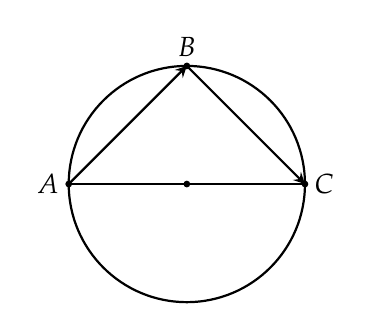
\begin{tikzpicture}[>=stealth]
	    
	    % Circle centered at (-1.2, 1.5) with radius 1.5
	    \draw[thick] (-1.2, 1.5) circle (1.5);
	    
	    % Mark the center
	    \filldraw (-1.2, 1.5) circle (1pt);
	    
	    % Points on the circle
	    \filldraw (-2.7, 1.5) circle (1pt) node[left] {$A$}; % Point A
	    \filldraw (0.3, 1.5) circle (1pt) node[right] {$C$}; % Point C
	    \filldraw (-1.2, 3) circle (1pt) node[above] {$B$}; % Point B
	    
	    % Draw diameter AC
	    \draw[thick] (-2.7, 1.5) -- (0.3, 1.5);
	    
	    % Draw line AB
	    \draw[thick, ->] (-2.7, 1.5) -- (-1.2, 3);
	    
	    % Draw line BC
	    \draw[thick, ->] (-1.2, 3) -- (0.3, 1.5);
	    
	    \end{tikzpicture}
	\end{center}

\vspace{-0.7cm}

Tú phải chèo thuyền đến gặp Thắng trước ở vị trí $ B $ trước rồi sau đó mới đi bộ đến vị trí $ C $. Tính thời gian di chuyển lâu nhất mà Tú có thể đi được biết rằng vận tóc chèo thuyền là $ 2 $ km/h và vận tốc đi bộ là $ 4 $ km/h (đơn vị giờ, kết quả làm tròn tới hàng phần trăm).

	\textit{\textbf{Đáp số: }}
	\framebox[20mm]{\rule{0pt}{4mm}}


\textbf{Câu 6: } Lúc 6 giờ 00 phút sáng kim phút và kim giờ tạo thành hai tia đối nhau. Biết rằng sau ít nhất $ x $ phút thì kim phút và kim giờ lại tạo thành hai tia đối nhau. Hỏi $ x $ bằng bao nhiêu phút (làm tròn đến hàng phần mười)

	\textit{\textbf{Đáp số: }}
	\framebox[20mm]{\rule{0pt}{4mm}}


\end{document}